\documentclass{beamer}

\usepackage[utf8]{inputenc}
\usepackage[ngerman]{babel}

\mode<presentation> {
  %\setbeameroption{show notes} % Kommentare im fertigen PDF

  \usetheme{Boadilla}
  \usecolortheme{seagull}

  \setbeamertemplate{footline}[page number] % Einfacher Folienzähler als Fußzeile
  \setbeamertemplate{navigation symbols}{} % Keine Navigationslinks
}

\title{Theoreme für lau!}
\author{Tim Baumann}
\institute[CCA]{Curry Club Augsburg}
\date{18. Mai 2017}

\usepackage{proof}

%\usepackage[outputdir=output]{minted} % Syntax-Highlighted Code; requires pygments to be installed
%\newminted[frankcode]{agda}{}
%\newmintinline[frankinline]{haskell}{}

\usepackage{hyperref}
%\usepackage{graphicx}

\newcommand{\defeq}{:=} % Definitionsgleich
\newcommand{\defiff}{:\xLeftrightarrow{\quad}} % Definitionsäquivalent
\newcommand{\IsType}[1]{{#1}\,\,\text{type}}
\newcommand{\IsCtx}[1]{{#1}\,\,\text{ctx}}
\newcommand{\Bool}{\text{Bool}}
\newcommand{\trueV}{\text{true}}
\newcommand{\falseV}{\text{false}}
\newcommand{\fa}[1]{\forall {#1}.\,}
\newcommand{\lam}[1]{\lambda #1.\,}
\newcommand{\Lam}[1]{\Lambda #1.\,}
\newcommand{\Types}{\text{Types}}
\newcommand{\Terms}{\text{Terms}}
\newcommand{\emptyCtx}{\bullet}
\newcommand{\blank}{\text{--}} % Platzhalter
\newcommand{\reducesTo}{\mathbin{\rightsquigarrow}} % Reduktionsrelation
\newcommand{\ite}[3]{\text{\textbf{if }} #1 \text{\textbf{ then }} #2 \text{\textbf{ else }} #3}
\newcommand{\obs}{\cong} % Observational equivalence

\usepackage{mathtools}
\usepackage{stmaryrd}
\DeclarePairedDelimiterX\Set[2]{\lbrace}{\rbrace}{ #1 \,\delimsize|\, #2 }
\DeclarePairedDelimiterX\interp[1]{\llbracket}{\rrbracket}{ #1 }

\newcommand{\typeInterp}[2]{\interp{#2}_{#1}}
\newcommand{\termInterp}[3]{\interp{#3}_{#1, #2}}
\newcommand{\relInterp}[2]{\interp{#2}_{#1}}
\newcommand{\Rel}[3]{#1 : #2 \Leftrightarrow #3}
%\newcommand{\funRel}[1]{\mathcal{R}_{#1}}
%\newcommand{\funRel}[1]{\xmapsto{#1}}
\newcommand{\funRel}[1]{\mathbin{|#1\rangle}}

% Populäre Typen
\DeclareMathOperator{\Sum}{Sum}
\DeclareMathOperator{\Product}{Product}
\DeclareMathOperator{\List}{List}
\DeclareMathOperator{\Nat}{Nat}

% Populäre Funktionen
\DeclareMathOperator{\fmap}{fmap}
\DeclareMathOperator{\id}{id}
\DeclareMathOperator{\pair}{pair}
\DeclareMathOperator{\nullF}{null}
\DeclareMathOperator{\append}{append}
\DeclareMathOperator{\map}{map}

% Färbe \emph{} violett
\usepackage{color,xcolor,graphicx,overpic}
%\definecolor{Emph}{rgb}{0.2,0.2,0.8}
\definecolor{Emph}{rgb}{0.52,0.078,0.294}
\renewcommand{\emph}[1]{\textcolor{Emph}{#1}}

\definecolor{dimgray}{rgb}{0.41, 0.41, 0.41}
\newcommand{\info}[1]{\textcolor{dimgray}{#1}}

\usefonttheme[onlymath]{serif}
\usepackage{eulervm}

% % Färbe Gleichungen rot
% \usepackage{everysel}
% \EverySelectfont{\color{black}}
% \definecolor{Maroon}{rgb}{0.52,0.078,0.294}
% \let\equation\gather
% \let\endequation\endgather
% \everymath{\color{Maroon}}
% %\everydisplay{\color{red}}

\newtheorem*{satz}{Satz}
\newtheorem*{lem}{Lemma}

% Macros copied from
% https://github.com/jonsterling/latex-common-notation
% https://github.com/jonsterling/forcing-bar-induction-in-system-t/blob/2bc8c69d849f03579470e5668e6b2a98af6c8054/macros.sty
\newlength{\jmssavedboxsep}
\newcommand\DeclBox[1]{%
  \setlength{\jmssavedboxsep}{\fboxsep}%
  \setlength{\fboxsep}{1.5pt}%
  \fcolorbox{black!50}{white}{$\displaystyle #1$}%
  \setlength{\fboxsep}{\jmssavedboxsep}%
}

\newcommand\DeclJdg[2]{\DeclBox{#1 \textit{ vorausgesetzt } #2}}

\begin{document}

\begin{frame}
  \titlepage
\end{frame}

\begin{frame}
  \begin{center}
    
\includegraphics[height=7cm]{wadler-lambdaman.jpg} \quad
    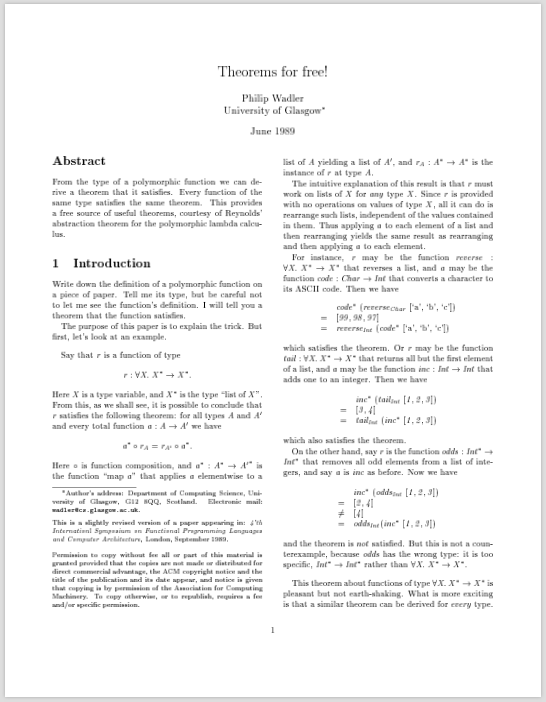
\includegraphics[height=7cm]{theorems-for-free.png}
  \end{center}
\end{frame}

\begin{frame}
  \begin{center}
    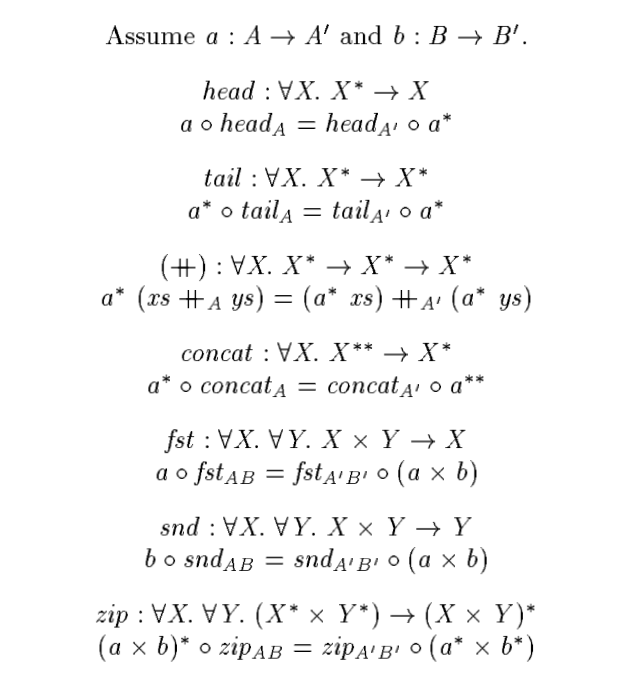
\includegraphics[scale=0.35]{theorems1.png}
  \end{center}
\end{frame}

\begin{frame}
  \frametitle{System F a.k.a. Girard–Reynolds polymorphic $\lambda$-calculus}

  \visible<1->{Die Typen von System~F sind durch die induktive Definition
  \[
    \tau \defeq \Bool \,|\, X \,|\, \tau_1 \to \tau_2 \,|\, \fa{X} \tau'
  \]
  gegeben, wobei $X$ für eine Typvariable steht.}
  \visible<2->{Ein \emph{Typkontext} ist eine endliche Menge $\Delta = \{ X_1, \ldots, X_n \}$ von Typvariablen.}
  \visible<3->{Die Typen im Typkontext~$\Delta$ sind die Typen, deren freie Variablen in~$\Delta$ liegen. Formal:
  \begin{gather*}
    \DeclBox{\Delta \vdash \IsType{\tau}} \qquad
    \infer{
      \Delta \vdash \IsType{\Bool}
    }{} \qquad
    \infer{
      \Delta \vdash \IsType{X}
    }{
      X \in \Delta
    } \\[0.4cm]
    \infer{
      \Delta \vdash \IsType{\tau_1 \to \tau_2}
    }{
      \Delta \vdash \IsType{\tau_1} \quad
      \Delta \vdash \IsType{\tau_2}
    } \qquad
    \infer{
      \Delta \vdash \IsType{\fa{X} \tau}
    }{
      \Delta \cup \{ X \} \vdash \IsType{\tau}
    }
  \end{gather*}}
\end{frame}

\begin{frame}
  \frametitle{Church-Kodierung in System F}
  \[\begin{array}{r c l}
    \Product(A, B) &\defeq& \fa{Y} (A \to B \to Y) \to Y \\
    \Sum(A, B) &\defeq& \fa{Y} (A \to Y) \to (B \to Y) \to Y \\
    \Nat &\defeq& \fa{Y} Y \to (Y \to Y) \to Y \\
    \List(A) &\defeq& \fa{Y} Y \to (A \to Y \to Y) \to Y \\
    \visible<2->{\Bool'(A) &\defeq& \fa{Y} Y \to Y \to Y}
  \end{array}\]
\end{frame}

\begin{frame}[t]
  \frametitle{Terme in System F}

  Die Terme~$t$ in System F sind induktiv definiert durch
  \[
    t \defeq \trueV \,|\, \falseV \,|\, \ite{t_1}{t_2}{t_3} \,|\, \lam{x{:}\tau} t \,|\, t_1\,t_2 \,|\, \Lam{A} t \,|\, t\,\tau
  \]

  \begin{onlyenv}<2-3>
  \visible<2-3>{Ein \emph{Wertekontext} ist eine endliche Menge $\Gamma = \{ x_1 : \tau_1, \ldots, x_m : \tau_m \}$, wobei $x_1, \ldots, x_m$ paarweise verschiedene \emph{Typvariablen} sind und $\tau_1, \ldots, \tau_m$ Typen sind.}
  \visible<3>{Er bildet zusammen mit~$\Delta$ einen \emph{Kontext} $\Delta; \Gamma$ falls die freien Variablen der Typen $\tau_1, \ldots, \tau_m$ in~$\Delta$ liegen. Formal:
  \[
    \DeclBox{\IsCtx{(\Delta; \Gamma)}} \qquad
    \infer{
      \IsCtx{(\Delta; {\emptyCtx})}
    }{} \qquad
    \infer{
      \IsCtx{(\Delta; \Gamma \cup \{x : \tau\})}
    }{
      \IsCtx{(\Delta; \Gamma)} \qquad
      \Delta \vdash \IsType{\tau}
    }
  \]}
  \end{onlyenv}

  \begin{onlyenv}<4->
  Ein Term $t$ hat Typ~$\tau$ in einem Kontext $\Delta; \Gamma$ (notiert $\Delta; \Gamma \vdash t : \tau$), falls
  \[ \DeclJdg{\Delta; \Gamma \vdash t : \tau}{\IsCtx{(\Delta; \Gamma)}} \qquad \]
  \[
    \infer{
      \Delta; \Gamma \vdash x : \tau
    }{
      (x : \tau) \in \Gamma
    }
  \]
  \[\begin{array}{c c}
    \infer{
      \Delta; \Gamma \vdash v : \Bool
    }{
      v \in \{ \trueV, \falseV \}
    } &
    \infer{
      \Delta; \Gamma \vdash \ite{b}{t}{e} : \tau
    }{
      \Delta; \Gamma \vdash b : \Bool \quad
      \Delta; \Gamma \vdash t : \tau \quad
      \Delta; \Gamma \vdash e : \tau
    } \\[0.3cm]
    \infer{
      \Delta; \Gamma \vdash \lam{x{:}\tau_1} t : \tau_1 \to \tau_2
    }{
      \Delta; \Gamma \cup \{ x : \tau_1 \} \vdash t : \tau_2
    } &
    \infer{
      \Delta; \Gamma \vdash f\,t : \tau_2
    }{
      \Delta; \Gamma \vdash f : \tau_1 \to \tau_2 \quad
      \Delta; \Gamma \vdash t : \tau_1
    } \\[0.3cm]
    \infer{
      \Delta; \Gamma \vdash \Lam{A} t : \fa{A} \tau
    }{
      \Delta \cup \{ A \}; \Gamma \vdash t : \tau
    } &
    \infer{
      \Delta; \Gamma \vdash t\,\tau : \tau'[\tau/A]
    }{
      \Delta; \Gamma \vdash t : \fa{A} \tau' \quad
      \Delta \vdash \IsType{\tau}
    }
  \end{array}\]
  \end{onlyenv}
\end{frame}

\begin{frame}[b]
  \frametitle{Beispielterme}
  \small
  \begin{align*}
    & \begin{array}{r l l}
      \id &:& \fa{A} A \to A \\
      \id &\defeq& \Lam{A} \lam{x{:}A} x
    \end{array} \\
    \visible<2->{
    & \begin{array}{r l l}
      \pair &:& \fa{A} \fa{B} A \to B \to \Product(A, B) \\
      \pair &\defeq& \Lam{A} \Lam{B} \lam{a{:}A} \lam{b{:}B} \\
      && \quad \Lam{Y} \lam{f{:}A \to B \to Y} \\
      && \quad\quad f\,a\,b
    \end{array} \\
    }\visible<3->{
    & \begin{array}{r l l}
      \nullF &:& \fa{A} \List(A) \to \Bool \\
      \nullF &\defeq& \Lam{A} \lam{xs{:}\List(A)} \\
      && \quad xs\,\Bool\,\trueV\,(\lam{a{:}A} \lam{b{:}\Bool} \falseV)
    \end{array} \\
    }\visible<4->{
    & \begin{array}{r l l}
      \append &:& \fa{A} \List(A) \to \List(A) \to \List(A) \\
      \append &\defeq& \Lam{A} \lam{xs{:}\List(A)} \lam{ys{:}\List(A)} \\
      && \quad \Lam{Y} \lam{y{:}Y} \lam{f{:}A \to Y \to Y} \\
      && \quad\quad ys\,Y\,(xs\,Y\,y\,f)\,f
    \end{array} \\
    }\visible<5->{
    & \begin{array}{r l l}
      \map &:& \fa{A} \fa{B} (A \to B) \to \List(A) \to \List(B) \\
      \map &\defeq& \Lam{A} \Lam{B} \lam{g{:}A \to B} \lam{xs{:}\List(A)} \\
      && \quad \Lam{Y} \lam{y{:}Y} \lam{f{:}B \to Y \to Y} \\
      && \quad\quad xs\,Y\,y\,(\lam{a{:}A} f\,(g\,a))
    \end{array}}
  \end{align*}
\end{frame}

\begin{frame}
  \frametitle{Reduktion und Äquivalenz von Termen in System F}
  Die Reduktionsrelation $\reducesTo$ auf der Menge der Terme ist die kleinste reflexive, transitive, kongruente Relation mit
  \[\begin{array}{r c l}
    \ite{\trueV}{t}{e} &\reducesTo& t \\
    \ite{\falseV}{t}{e} &\reducesTo& e \\
    (\lam{x} t) s &\reducesTo& t[s/x] \\
    (\Lam{X} t) \tau &\reducesTo& t[\tau/X]
  \end{array}\]

  \visible<2->{
  Zwei Terme $b, b' : \Bool$ heißen \emph{Kleene-äquivalent}, notiert $b \simeq b'$, falls
  \[
    b \simeq b'
    \enspace\defiff\enspace
    (t \reducesTo \trueV \iff t' \reducesTo \trueV).
  \]}

  \visible<3->{
  Sei $A$ ein Typ.
  Zwei Terme $t, t' \in A$ heißen \emph{beobachtungsäquivalent}, falls
  \[
    t \obs t'
    \enspace\defiff\enspace
    \text{für alle $f : A \to \Bool$ gilt $f\,t \simeq f\,t'$}.
  \]}
\end{frame}

\begin{frame}
  \frametitle{Interpretation von Typen}

  Eine \emph{Typumgebung} für einen Typkontext~$\Delta$ ist eine Abbildung
  \[ \vec{A} : \Delta \to \Types_\emptyCtx \]
  wobei wir $\Types_{\widetilde{\Delta}} \defeq \Set{\tau}{\widetilde{\Delta} \vdash \tau}$ für alle Typkontexte~$\widetilde{\Delta}$ definieren.\\[0.5cm]

  \begin{visibleenv}<2->
  Jede Typumg. $\vec{A}$ induziert für jeden disjunkten Typkontext~$\Delta'$ eine Abb.
  \[ \typeInterp{\vec{A}}{\blank} : \Types_{\Delta \sqcup \Delta'} \to \Types_{\Delta'} \]
  rekursiv definiert durch
  \[
    \begin{array}{r c l l}
      \typeInterp{\vec{A}}{\Bool} &\defeq& \Bool \\
      \typeInterp{\vec{A}}{X} &\defeq& \vec{A}(X) \text{ falls $X \in \Delta$} \\
      \typeInterp{\vec{A}}{X} &\defeq& X \text{ falls $X \in \Delta'$} \\
      \typeInterp{\vec{A}}{\tau_1 \to \tau_2} &\defeq& \typeInterp{\vec{A}}{\tau_1} \to \typeInterp{\vec{A}}{\tau_2} \\
      \typeInterp{\vec{A}}{\fa{X} \tau} &\defeq& \fa{X} \typeInterp{\vec{A}}{\tau} & \text{\info{(\OE{} $X \not\in \Delta \cup \Delta'$)}} \\
    \end{array}
  \]
  \end{visibleenv}
\end{frame}

\begin{frame}
  \frametitle{Relationen zwischen Typen}

  Eine \emph{Relation} $\Rel{\mathcal{A}}{A}{A'}$ zwischen zwei Typen $A, A' \in \Types_\bullet$ ist eine Relation zwischen den Termmengen dieser beiden Typen, für die gilt:
  \[
    \text{aus}\quad
    t_1 \obs t_2, \enspace
    t'_1 \obs t'_2
    \qquad\text{folgt}\qquad
    \mathcal{A}(t_1, t'_1) \iff
    \mathcal{A}(t_2, t'_2).
  \]

  \visible<2->{
    Wichtiges Beispiel:
    Seien $A$ und $B$ Typen und $f : A \to B$ eine Funktion.
    Dann definiert
    \[
      x \funRel{f} y \enspace\defiff\enspace f\,x \obs y
    \]
    eine Relation $\Rel{\funRel{f}}{A}{B}$.
  }
\end{frame}

\begin{frame}
  \frametitle{Relationen zwischen Typen}
  Eine \emph{Relation}~$\Rel{\vec{\mathcal{A}}}{\vec{A}}{\vec{A}'}$ zwischen Typumgebungen $\vec{A}$ und $\vec{A}'$ für~$\Delta$ ist eine Familie von Relationen
  \[ (\Rel{\mathcal{A}_X}{\vec{A}(X)}{\vec{A}'(X)})_{X \in \Delta}. \]
  %von Relationen zwischen den Typen $\vec{A}(X)$ und $\vec{A}'(X)$ für alle $X \in \Delta$.

  \visible<2->{Solch eine Relation $\Rel{\vec{\mathcal{A}}}{\vec{A}}{\vec{A}'}$ induziert für jeden Typ~$\tau$ im Typkontext~$\Delta$ eine Relation $\Rel{\relInterp{\vec{\mathcal{A}}}{\tau}}{\typeInterp{\vec{A}}{\tau}}{\typeInterp{\vec{A}'}{\tau}}$ wie folgt:
  \[
    \begin{array}{r c l}
      \relInterp{\vec{\mathcal{A}}}{\Bool} &\defeq& (\simeq) \\
      \relInterp{\vec{\mathcal{A}}}{X} &\defeq& \mathcal{A}_X \\
      \relInterp{\vec{\mathcal{A}}}{\tau_1 \to \tau_2} &\defeq& \relInterp{\vec{\mathcal{A}}}{\tau_1} \to \relInterp{\vec{\mathcal{A}}}{\tau_2} \\
      \relInterp{\vec{\mathcal{A}}}{\fa{X} \tau} &\defeq& \sim \text{ mit } g \sim g' \text{ genau dann wenn} \\
      && \quad \text{für alle $A, A' \in \Types_\emptyCtx$} \\
      && \quad \text{und Relationen $\Rel{\mathcal{A}}{A}{A'}$} \\
      && \quad \text{gilt } \relInterp{(\vec{\mathcal{A}} \cup \{X \mapsto \mathcal{A}\})}{\tau}(g\,A, g'\,A'),
    \end{array}
  \]
  wobei wir definieren:
  \[
    (\mathcal{R}_1 \to \mathcal{R}_2)(f, f') \defiff
    \text{für alle $a$, $a'$ mit $\mathcal{R}_1(a, a')$ gilt $\mathcal{R}_2(f\,a, f'\,a')$}.
  \]}
\end{frame}

\begin{frame}
  \begin{satz}[Parametrizität]
    Für jeden Typ $\tau \in \Types_\emptyCtx$ und jeden Term $t : \tau$ gilt $\relInterp{\emptyCtx}{\tau}(t, t)$
  \end{satz}

  \begin{satz}<2->
    Für jeden Typ $\tau \in \Types_\emptyCtx$ und Terme $t, t' \in \tau$ gilt
    \[
      t \obs t' \iff \relInterp{\emptyCtx}{\tau}(t, t').
    \]
  \end{satz}
\end{frame}

\begin{frame}[t]
  \frametitle{Ein Isomorphismus}
  Sei $A$ ein Typ. Definiere $\widehat{A} \defeq \fa{Y} (A \to Y) \to Y$.
  Wir haben Funktionen
  \[\begin{array}{l l}
    i : A \to \widehat{A}, & i \defeq \lam{x{:}A} \Lam{Y} \lam{g{:}A \to Y} g\,x \\
    j : \widehat{A} \to A, & j \defeq \lam{h{:}\widehat{A}} h\,A\,(\id\,A)
  \end{array}\]
  \visible<2->{Es gilt $j\,(i\,x) \reducesTo x$, also $j\,(i\,x) \obs x$, aber stimmt auch $i\,(j\,h) \obs h$?}
  \visible<3->{Parametricity to the rescue!
  Für $h : \widehat{A}$, $f : A \to B$ und $b : B \to B'$ gilt}
  \begin{onlyenv}<4-10>
  \[\begin{array}{r l}
    \visible<4->{
      & \relInterp{\emptyCtx}{\widehat{A}}(h, h) \\
    }
    \visible<5->{
      \iff & \text{für alle $S, S'$ und $\Rel{\mathcal{S}}{S}{S'}$ gilt $\relInterp{\{ Y \mapsto \mathcal{S} \}}{(A \!\to\! Y) \!\to\! Y}(h\,S, h\,S')$} \\
    }
    \visible<6->{
      \implies & \relInterp{\{ Y \mapsto \funRel{b} \}}{(A \to Y) \to Y}(h\,B, h\,B') \\
    }
    \visible<7->{
      \iff & \text{für alle $g : A \to B$, $g' : A \to B'$ mit \only<7>{$\relInterp{\{ Y \mapsto \funRel{b} \}}{A \to Y}(g, g')$}\only<8->{$b\,(g\,a) = g'\,a$ f.\,a. $a \in A$}} \\
      & \text{gilt $\relInterp{\{ Y \mapsto \funRel{b} \}}{Y}(h\,B\,g, h\,B'\,g')$} \\
    }
    \visible<9->{
      \implies & \text{$\relInterp{\{ Y \mapsto \funRel{b} \}}{Y}(h\,B\,f, h\,B'\,(b \circ f))$} \\
    }
    \visible<10->{
      \iff & b\,(h\,B\,f) \obs h\,B'\,(b \circ f)
    }
  \end{array}\]
  \end{onlyenv}
  \begin{onlyenv}<11->
    \[ b\,(h\,B\,f) \obs h\,B'\,(b \circ f). \]
  \end{onlyenv}
  \begin{onlyenv}<12->
  Es folgt mit $B = A$, $B' = X$, $b = g$ und $f = \id\,A$:
  \[\begin{array}{r c l}
    i\,(j\,h) &\obs& \Lam{X} \lam{g{:}A \to X} g\,(h\,A\,(\id\,A)) \\
    \visible<12->{&\obs& \Lam{X} \lam{g{:}A \to X} h\,X\,(g \circ (\id\,A)) \\}
    \visible<13->{&\obs& \Lam{X} \lam{g{:}A \to X} h\,X\,g \\}
    \visible<14->{&\obs& h}
  \end{array}\]
  \end{onlyenv}
\end{frame}

\begin{frame}[t]
  \frametitle{Das zweite Funktoraxiom}
  \begin{onlyenv}<1-8>
  Sei $F(X)$ ein über~$X$ parametrisierter Typ, (d.h.\,$X \vdash F(X)$) und gelte, dass $X$ in $F(X)$ nur kovariant vorkommt.
  \begin{lem}<2->
    Für alle $A, B \in \Types_\bullet$ und $f : A \to B$ gibt es eine Funktion $f_* : F(A) \to F(B)$, sodass für alle $a : F(A)$ und $b : F(B)$ gilt:
    \[
      \relInterp{\{ X \mapsto \funRel{f} \}}{F(X)}(a, b)
      \enspace\iff\enspace
      f_*(a) \obs b
    \]
  \end{lem}
  \end{onlyenv}
  \visible<3->{Seien $\fmap : \fa{X} \fa{Y} (X \to Y) \to (F(X) \to F(Y))$, Typen $A, A', B, B'$ und Funktionen $f_1 : A \to A'$, $f_2 : A' \to B'$, $g_1 : A \to B$, $g_2 : B \to B'$ mit $f_2 \circ f_1 \obs g_2' \circ g_1$ sowie $p : F(A)$ gegeben.
  Dann gilt:}
  \begin{onlyenv}<4-8>\[\begin{array}{r l}
    \visible<4->{
      & \relInterp{\emptyCtx}{\fa{X} \fa{Y} (X \to Y) \to (F(X) \to F(Y)}(\fmap, \fmap) \\
      %\implies & \relInterp{\{ X \mapsto \funRel{f_1} \}}{\fa{Y} (X \!\to\! Y) \!\to\! (F(X) \!\to\! F(Y)}(\fmap\,A, \fmap\,A') \\
    }
    \visible<5->{
      \implies & \relInterp{\{ X \mapsto \funRel{f_1}, Y \mapsto \funRel{g_2} \}}{(X \!\to\! Y) \!\to\! (F(X) \!\to\! F(Y)}(\fmap\,A\,B, \fmap\,A'\,B') \\
    }
    \visible<6->{
      \implies & \relInterp{\{ X \mapsto \funRel{f_1}, Y \mapsto \funRel{g_2} \}}{F(X) \!\to\! F(Y)}(\fmap\,A\,B\,g_1, \fmap\,A'\,B'\,f_2) \\
    }
    \visible<7->{
      \implies & \relInterp{\{ X \mapsto \funRel{f_1}, Y \mapsto \funRel{g_2} \}}{F(Y)}(\fmap\,A\,B\,g_1\,p, \fmap\,A'\,B'\,f_2\,((f_1)_*\,p)) \\
    }
    \visible<8->{
      \iff & (g_2)_*\,(\fmap\,A\,B\,g_1\,p) \obs \fmap\,A'\,B'\,f_2\,((f_1)_*\,p)
    }
  \end{array}\]\end{onlyenv}\begin{onlyenv}<9->
  \[ (g_2)_* \circ \fmap\,A\,B\,g_1 \obs \fmap\,A'\,B'\,f_2 \circ (f_1)_* \]
  \visible<11->{
    Angenommen, für alle Typen~$A$ gilt $\fmap\,A\,A\,(\id\,A) \obs \id\,F(A)$.
  }

  \visible<12->{Dann gilt für alle Funktionen $f : A \to B$:}
  \[
    \visible<13->{\fmap\,A\,B\,f \obs (\id\,B)_* \circ \fmap\,A\,B\,f
    \obs \fmap\,B\,B\,(\id\,B) \circ f_* \obs f_*}
  \]
  \visible<13->{Für Typen $C, D, E$ und Funktionen $k : C \to D$ und $h : D \to E$ folgt:}
  \[\begin{array}{r c l}
    \visible<14->{
      \fmap\,D\,E\,h \circ \fmap\,C\,D\,k
    }
    \visible<15->{
      &\obs& h_* \circ \fmap\,C\,D\,k \\
    }
    \visible<16->{
      &\obs& \fmap\,E\,E\,(\id\,E) \circ (h \circ k)_* \\
    }
    \visible<17->{
      &\obs& (h \circ k)_* \\
    }
    \visible<18->{
      &\obs& \fmap\,C\,E\,(h \circ k) \\
    }
  \end{array}\]
  \begin{center}
    \visible<19->{\textbf{Fazit: Das zweite Funktoraxiom ist kostenlos!}}
  \end{center}
  \end{onlyenv}
\end{frame}

\begin{frame}[t]
  \frametitle{Sortierfunktionen}
  Angenommen, wir haben $s : \fa{X} (X \to X \to \Bool) \to \List(X) \to \List(X)$, $c' : B' \to B' \to \Bool$, $f : B \to B'$ und $bs : \List(B)$. \\
  Definiere $c \defeq (\lam{x{:}B} \lam{y{:}B} c\,(f\,x)\,(f\,y)) : B \to B \to \Bool$.
  Dann gilt
  \[\begin{array}{r l}
    & \relInterp{\emptyCtx}{\fa{X} (X \to X \to \Bool) \to \List(X) \to \List(X)}(s, s) \\
    \visible<2->{
      \iff & \text{für alle $S, S'$, $\Rel{\mathcal{S}}{S}{S'}$ gilt} \\
      & \relInterp{\{ X \mapsto \mathcal{S} \}}{(X \to X \to \Bool) \to \List(X) \to \List(X)}(s\,S, s\,S') \\
    }
    \visible<3->{
      \implies & \relInterp{\{ X \mapsto \funRel{f} \}}{(X \to X \to \Bool) \to \List(X) \to \List(X)}(s\,B, s\,B') \\
    }
    \visible<4->{
      \iff & \text{für alle $g : A \to A \to \Bool$, $g' : B' \to B' \to \Bool$} \\
      & \text{mit $\relInterp{\{X \mapsto \funRel{f}\}}{X \to X \to \Bool}(g, g')$} \\
      & \text{gilt } \relInterp{\{ X \mapsto \funRel{f} \}}{\List(X) \to \List(X)}(s\,B\,g, s\,B'\,g') \\
    }
    \visible<5->{
      \implies & \relInterp{\{ X \mapsto \funRel{f} \}}{\List(X) \to \List(X)}(s\,B\,c, s\,B'\,c') \\
    }
    \visible<6->{
      \iff & \text{für alle $xs : \List(B)$, $ys : \List(B')$ mit $\relInterp{\{ X \mapsto \funRel{f} \}}{\List(X)}(xs, ys)$} \\
      & \text{gilt } \relInterp{\{ X \mapsto \funRel{f} \}}{\List(X)}(s\,B\,c\,xs, s\,B'\,c'\,ys) \\
    }
    \visible<7->{
      \implies & \relInterp{\{ X \mapsto \funRel{f} \}}{\List(X)}(s\,B\,c\,bs, s\,B'\,c'\,(\text{map}\,B\,B'\,f\,bs)) \\
    }
    \visible<8->{
      \iff & \text{map}\,B\,B'\,f\,(s\,B\,c\,bs) \obs s\,B'\,c'\,(\text{map}\,B\,B'\,f\,bs)
    }
  \end{array}\]
\end{frame}

\begin{frame}
  \frametitle{Natürlichkeit}
  Seien $F(X)$ und $G(X)$ über $X$ parametrisierte Typen (wie eben) und $eta : \fa{Y} F(Y) \to G(Y)$ eine Funktion.

  \visible<2->{Beispiele in Haskell: maybeToList, reverse, maybeHead}

  \visible<3->{Für alle Typen $A$, $A'$ und Funktionen $f : A \to A'$ folgt aus Parametrizität:}
  \[\begin{array}{r l}
    \visible<3->{
      & \relInterp{\emptyCtx}{\fa{Y} F(Y) \to G(Y)}(eta, eta) \\
    }
    \visible<4->{
      \implies & \relInterp{\{ Y \mapsto \funRel{f} \}}{F(Y) \to G(Y)}(eta\,A, eta\,A') \\
    }
    \visible<5->{
      \iff & \text{für alle $a : A$ und $a' : A'$ mit $\relInterp{\{ Y \mapsto \funRel{f} \}}{F(Y)}(a, a')$} \\
      & \text{gilt } \relInterp{\{ Y \mapsto \funRel{f} \}}{G(Y)}(eta\,A\,a, eta\,A'\,a') \\
    }
    \visible<6->{
      \iff & \text{für alle $a : A$ und $a' : A'$ mit $f_*\,a \obs a'$} \\
      & \text{gilt } f_*\,(eta\,A\,a) \obs eta\,A'\,a' \\
    }
    \visible<7->{
      \iff & f_* \circ eta\,A \obs eta\,A' \circ f_* \\
    }
  \end{array}\]
  \begin{center}
    \visible<8->{\textbf{Fazit: Natürlichkeit ist kostenlos!}}
  \end{center}
\end{frame}

\begin{frame}
  \frametitle{Beweis von Parametrizität: Interpretation von Termen}

  Eine \emph{Termumgebung} $\vec{a}$ für einen Kontext $\Delta; \Gamma$ bzgl. einer Typumgebung $\vec{A}$ für~$\Delta$ ist eine Familie
  \[ (\vec{a}(x) : \typeInterp{\vec{A}}{\tau})_{(x : \tau) \in \Gamma}. \]
  von Termen.
  \visible<2->{Jede solche Termumgebung induziert für jeden von $\Delta;\Gamma$ disjunkten Kontext $\Delta';\Gamma'$ eine Interpretationsabbildung
  \[ \termInterp{\vec{A}}{\vec{a}}{\blank} : \Terms_{\Delta \sqcup \Delta', \Gamma \sqcup \Gamma'} \to \Terms_{\Delta', \Gamma'} \]
  rekursiv definiert durch
  \[
    \begin{array}{r c l l}
      \termInterp{\vec{A}}{\vec{a}}{v} &\defeq& v & \info{(v \in \{ \trueV, \falseV \})} \\
      \termInterp{\vec{A}}{\vec{a}}{\ite{b}{t}{e}} &\defeq& \mathrlap{\ite{\termInterp{\vec{A}}{\vec{a}}{b}}{\termInterp{\vec{A}}{\vec{a}}{t}}{\termInterp{\vec{A}}{\vec{a}}{e}}} \\
      \termInterp{\vec{A}}{\vec{a}}{\lam{x{:}\tau} t} &\defeq& \lam{x{:}\typeInterp{\vec{A}}{\tau}} \termInterp{\vec{A}}{\vec{a}}{t} & \text{\info{(\OE{} $x \not\in \Gamma \cup \Gamma'$)}} \\
      \termInterp{\vec{A}}{\vec{a}}{t_1 \, t_2} &\defeq& \termInterp{\vec{A}}{\vec{a}}{t_1} \, \termInterp{\vec{A}}{\vec{a}}{t_2} \\
      \termInterp{\vec{A}}{\vec{a}}{\Lam{X} t} &\defeq& \Lam{X} \termInterp{\vec{A}}{\vec{a}}{t} & \text{\info{(\OE{} $X \not\in \Delta \cup \Delta'$)}} \\
      \termInterp{\vec{A}}{\vec{a}}{t\,\tau} &\defeq& \termInterp{\vec{A}}{\vec{a}}{t}\,\typeInterp{\vec{A}}{\tau} \\
    \end{array}
  \]}
\end{frame}

\begin{frame}
  \frametitle{Beweis von Parametrizität}

  Seien $\vec{A}$ und $\vec{A}'$ Typumgebungen für~$\Delta$, $\Rel{\vec{\mathcal{A}}}{\vec{A}}{\vec{A}'}$ eine Relation.
  Zwei Termumg. $\vec{a}$ und $\vec{A}'$ für $\Delta; \Gamma$ bzgl. $\vec{A}$ bzw.~$\vec{A}'$ sind \emph{relatiert} bzgl. $\vec{\mathcal{A}}$, falls
  \[
    \relInterp{\vec{\mathcal{A}}}{\tau}(\vec{a}(x), \vec{A}'(x))
    \quad \text{für alle $(x : \tau) \in \Gamma$}.
  \]
  \[
    \arraycolsep=2pt
    \begin{array}{r c l l}
    \Delta; \Gamma \models t : \tau &\defiff
    &\text{für}& \text{alle Typumgebungen $\vec{A}$, $\vec{A}'$ von~$\Delta$ und} \\
    &&& \text{alle Relationen $\Rel{\vec{\mathcal{A}}}{\vec{A}}{\vec{A}'}$ und} \\
    &&& \text{alle relatierten Termumg. $\vec{a}$ bzgl.~$\vec{A}$ und $\vec{A}'$ bzgl. $\vec{A}'$} \\
    &&\text{gilt}& \relInterp{\vec{\mathcal{A}}}{\tau}(\termInterp{\vec{A}}{\vec{a}}{t}, \termInterp{\vec{A}'}{\vec{A}'}{t})
  \end{array}
  \]

  \visible<2->{\begin{satz}[Parametrizität']
    Aus $\Delta; \Gamma \vdash t : \tau$ folgt $\Delta; \Gamma \models t : \tau$
  \end{satz}}

  \visible<3->{Kurz: Interpretationen in relatierten Umgebungen sind relatiert.}
\end{frame}

\begin{frame}
  \[
    \infer{
      \Delta; \Gamma \models x : \tau
    }{
      (x : \tau) \in \Gamma
    }
  \]
  \[\begin{array}{c c}
    \infer{
      \Delta; \Gamma \models v : \Bool
    }{
      v \in \{ \trueV, \falseV \}
    } &
    \infer{
      \Delta; \Gamma \models \ite{b}{t}{e} : \tau
    }{
      \Delta; \Gamma \models b : \Bool \quad
      \Delta; \Gamma \models t : \tau \quad
      \Delta; \Gamma \models e : \tau
    } \\[0.3cm]
    \infer{
      \Delta; \Gamma \models \lam{x{:}\tau_1} t : \tau_1 \to \tau_2
    }{
      \Delta; \Gamma \cup \{ x : \tau_1 \} \models t : \tau_2
    } &
    \infer{
      \Delta; \Gamma \models t_1\,t_2 : \tau_2
    }{
      \Delta; \Gamma \models t_1 : \tau_1 \to \tau_2 \quad
      \Delta; \Gamma \models t_2 : \tau_1
    } \\[0.3cm]
    \infer{
      \Delta; \Gamma \models \Lam{A} t : \fa{A} \tau
    }{
      \Delta \cup \{ A \}; \Gamma \models t : \tau
    } &
    \infer{
      \Delta; \Gamma \models t\,\tau : \tau'[\tau/A]
    }{
      \Delta; \Gamma \models t : \fa{A} \tau' \quad
      \Delta \vdash \IsType{\tau}
    }
  \end{array}\]
\end{frame}

\begin{frame}
  \frametitle{Links und Quellen}
  \begin{itemize}
    \item \url{http://twitter.com/parametricity}
    \item Free Theorems Web-UI: \url{http://www-ps.iai.uni-bonn.de/cgi-bin/free-theorems-webui.cgi}
    \item Philip Wadler, \textit{Theorems for Free!}, 4'th International Conference on Functional Programming and Computer Architecture, London, September 1989
    \item Robert Harper, \textit{Practical Foundations for Programming Languages}, zweite Auflage, Kapitel 48
    \item Edward Kmett, \textit{The free theorem for fmap}, \url{https://www.schoolofhaskell.com/user/edwardk/snippets/fmap}
  \end{itemize}
\end{frame}

\end{document}